% Preamble
% =============================================================================

% Class of the document.
\documentclass[12pt,a4paper]{article}
% article : short article.
% report  : mid-length report.
% book    : book or thesis redaction.

% Paragraph skip length (default to 0).
\setlength{\parskip}{1ex}

% Packages
% =============================================================================

% Encoding
% -----------------------------------------------------------------------------

% Babel.
\usepackage[french]{babel}
% FontEnc.
\usepackage[T1]{fontenc}
% InputEnc.
\usepackage[utf8]{inputenc}

% Define \escapeus command to escape underscores.
\makeatletter
\DeclareRobustCommand*{\escapeus}[1]{
    \begingroup\@activeus\scantokens{#1\endinput}\endgroup}
\begingroup\lccode`\~=`\_\relax
    \lowercase{\endgroup\def\@activeus{\catcode`\_=\active \let~\_}}
\makeatother

% Text
% -----------------------------------------------------------------------------

% Acronym.
\usepackage{acronym}
% CsQuote.
\usepackage[style=french,french=guillemets]{csquotes}
% Enumerate.
\usepackage{enumerate}
% HyperRef.
\usepackage[hyperfootnotes=false,hidelinks]{hyperref}
% URL.
\usepackage{url}

% Algorithms
% -----------------------------------------------------------------------------

% Algorithm2E.
\usepackage[french,onelanguage,linesnumbered,ruled,vlined,commentsnumbered]{algorithm2e}

% Source code
% -----------------------------------------------------------------------------

% Listings.
\usepackage{listings}
% Minted.
\usepackage{minted}
% Caption.
\usepackage{caption}
\newenvironment{code}{\captionsetup{type=listing}}{}

% Files
% -----------------------------------------------------------------------------

% FancyVRB.
\usepackage{fancyvrb}
% Redefine \VerbatimInput.
\RecustomVerbatimCommand{\VerbatimInput}{VerbatimInput}
{
    fontsize=\footnotesize,
    frame=lines,         % Top and bottom rule only.
    framesep=1.5em,      % Separation between frame and text.
    rulecolor=\color{red!50!green!50!blue!50!},
    labelposition=topline,
    commandchars=\|\(\), % Escape character and argument delimiters for commands within the verbatim.
    commentchar=*        % Comment character.
}

% Figures
% -----------------------------------------------------------------------------

% GraphicX.
\usepackage{graphicx}
% SVG.
\usepackage{svg}
% WrapFig.
\usepackage{wrapfig}

% Charts
% -----------------------------------------------------------------------------

% PGFPLots
\usepackage{pgfplots}
\pgfplotsset{compat=1.16}
\usepgfplotslibrary{units}

% Mathematics
% -----------------------------------------------------------------------------

% AmsFonts.
\usepackage{amsfonts}
% AmsMath.
\usepackage{amsmath}
% AmsText.
\usepackage{amstext}
% AmsThm.
\usepackage{amsthm}
\newtheorem{prr}{Propriété}
\newtheorem{pro}{Proposition}
\newtheorem{thm}{Théorème}
\newtheorem{lem}{Lemme}
% NumPrint.
\usepackage{numprint}

% Physics
% -----------------------------------------------------------------------------

% Physics.
\usepackage{physics}

% Presentation
% -----------------------------------------------------------------------------

% XColor.
\usepackage{xcolor}

% References
% -----------------------------------------------------------------------------

% CleveRef.
\usepackage{cleveref}

% Structure.
% -----------------------------------------------------------------------------

% Geometry.
\usepackage{geometry}
% PDFLScape.
\usepackage{pdflscape}
% MultiCol.
\usepackage{multicol}
% TitleSec.
\usepackage{titlesec}
\newcommand{\sectionbreak}{\clearpage} % Use a page break before new sections.
% VMargin.
\usepackage{vmargin}
% FootMisc.
\usepackage[bottom]{footmisc}

% Symbols
% -----------------------------------------------------------------------------

% SIUnitX.
\usepackage{siunitx}

% Table
% -----------------------------------------------------------------------------

% Array.
\usepackage{array}
% BookTabs.
\usepackage{booktabs}
% CSVSimple.
\usepackage{csvsimple}

% Document
% =============================================================================

\begin{document}

\title{Analyse de performance et optimisation de code}
\author{Pierre AYOUB}

\maketitle

\begin{figure}[b]
    \centering
    
\includegraphics[scale=0.3]{figures/isty.jpg}
\end{figure}

\newpage
\begin{abstract}

La simulation numérique est un procédé informatique visant à modéliser un
phénomène par ordinateur, s’agissant le plus souvent d’un phénomène
physique. Cette modélisation prend forme par des systèmes d’équations
décrivant l’état du système physique représenté à chaque instant. De
nombreux domaines scientifiques convergent vers la simulation
informatique, tel que certaines branches de la physique, de l’analyse
et de l’optimisation mathématique, ou encore le calcul haute
performance en informatique. Enfin, la simulation trouve naturellement
de nombreuses applications concernant des sujets variés, tel que la
simulation du climat et des évènements météorologiques, la simulation
d’essais nucléaires, de l’effet d’un médicament sur un corps, ou encore
des astres et de l’univers. Ce rapport s’articulera donc autour de la
simulation de fumée, phénomène impliquant les lois de la mécanique des
fluides. Notre travail portera sur l’aspect du calcul haute performance
de cette simulation.

\end{abstract}

\tableofcontents

\section{Introduction}
\label{sec.intro}

Le projet que nous vous présentons aujourd’hui consiste à analyser puis,
grâce à nos mesures, optimiser un code de simulation numérique. Ce dernier
nous offre une interface graphique permettant d’ajouter de la fumée dans un
espace confiné et, ainsi, d’en observer le comportement. Nous pouvons
influencer la quantité de fumée et sa vélocité dans l’espace. De plus,
l’application nous donne le contrôle sur la résolution de la simulation,
cela revient à dire sur sa précision, qui détermine principalement la
performance du programme.

Le déroulement du projet s’est effectué en plusieurs étapes distinctes :
\begin{description}
    \item[Analyse du code] Cette phase consiste à analyser le programme
        d’un point de vue mathématique et informatique. De cette première
        approche, il s’agira de comprendre les opérations du programme sur
        les équations qui régissent le système physique. De l’autre
        approche, il convient d’étudier l’architecture logicielle de
        l’application, ainsi que les choix mis en œuvres afin d’implémenter
        le ou les algorithmes nécessaires.
    \item[Protocole expérimental] Une fois l’analyse effectuée, nous
        pouvons en déduire le moyen le plus adapté afin de mesurer les
        performances de notre implémentation. Nous allons donc mettre en
        avant les critères théoriques à atteindre dans nos mesures, puis
        nous exposerons la manière dont nous avons mis ceci en pratique.
    \item[Optimisations et mesures] Grâce au protocole mis en place, nous
        pouvons quantifier la performance du programme. De ce fait, nous serons
        en mesure d’expérimenter différentes techniques d’optimisation sur le
        programme et d’en calculer l’accélération.
\end{description}

\section{Analyse du code}
\label{sec.analyze}

% \VerbatimInput[label=\fbox{\color{red!85!green!85!blue!85!}fluid.cflow},]{figures/callgraph/fluid.cflow}

L'analyse du code est la première étape à effectuer afin d'optimiser un code. Il
s'agit d'identifier les différentes sections et fonctions qui pourraient être
critiques, ainsi que de comprendre mathématiquement quelles fonctions
remplissent quels rôles.

L’interface du programme et l’interaction avec l’utilisateur est géré par les
fichiers \enquote{demo.html}, \enquote{FluidSolver.java} et
\enquote{WebStart.java}. À priori, ces fichiers nous importe peu dans notre
processus d’analyse et d’optimisation. Le cœur de la simulation se déroule dans
le fichier \enquote{fluid.c}, dans lequel se situe les fonctions de calcul des
phénomènes physique.

\begin{figure}[h]
    \centering
    {
        \scriptsize
        \escapeus{\includesvg[scale=0.5]{figures/callgraph/fluid.svg}}
    }
    \caption{Graphe d'appel du fichier \textit{fluid.c}}
    \label{fig.analyze.callgraph}
\end{figure}

Avant d'observer et d’analyser attentivement le code du fichier
\enquote{fluid.c}, nous avons utilisé \textbf{Cflow} afin d’obtenir un graphe
d’appel pour avoir une vue d’ensemble et observer les liens entre les fonctions.
Le résultat est présenté dans la figure~\ref{fig.analyze.callgraph}. Nous
décrivons ici les fonctions principales. On remarque très rapidement les deux
points d’entrés du programme : \enquote{c\_densitySolver()} et
\enquote{c\_velocitySolver()}. Ces deux fonctions sont utilisées conjointement
pour assurer les deux fonctionnalités de notre simulation : la première permet
de calculer la position d’une particule de fumée ajouté par la souris, la
deuxième permet de calculer leur déplacement en fonction des différentes
vélocités dans l’espace. Nous observons ensuite deux fonctions qui sont ici pour
assurer des opérations physique : \enquote{project()} et \enquote{diffuse()}. Le
nom laisse sous entendre que la première permet de faire une projection (des
coordonnées d’un système à un autre ?) et la seconde permet de diffuser (une
particule dans l’espace ?), mais nos connaissances en mécanique des fluides nous
arrêtent ici pour les suppositions. Cependant, il est intéressant d’observer que
ces deux fonctions font appel à une nouvelle fonction :
\enquote{linearSolver()}. Cette fonction, comme le nom le laisse entendre, est
le cœur de calcul de l’application : elle permet de résoudre un système
d’équation linéaire. Il ne fait aucune doute que c’est dans cette fonction que
de nombreuses optimisations seront possibles ! Enfin, on observe quelques autres
fonctions de physique (\enquote{vorticityConfinement()}, \enquote{advect()},
\enquote{buoyancy()}) ou des fonctions de mathématiques (\enquote{sqrt()},
\enquote{abs()}) qui gravitent autour des fonctions précédemment décrites.
Enfin, une fonction semble être appelée par quasiment toutes les autres de
manière récursive : la fonction \enquote{build\_index()} . Cette fonction, très
courte, permet de passer d’un couple de coordonnées $(i, j)$ identifiant une
donnée à un offset correspondant à son emplacement mémoire par rapport à la base
de la matrice. Cette fonction, présente à de nombreux endroits dans le code,
devrait aussi avoir droit à une attention particulière.

\section{Protocole expérimental}
\label{sec.prot}

La mise en place d’un protocole expérimental de mesure est une étape nécessaire
et cruciale dans tout optimisation de code. D’une part, le but de ce protocole
est de mettre en lumière les points chauds du programme, c’est-à-dire les
parties du code qui ralentissent considérablement l’exécution de la simulation.
Ces points chauds seront les cibles de nos optimisations. D’autre part, après
chaque tentative d’optimisation, le protocole doit nous permettre de mesurer
l’impact de cette dernière, qu’il soit positif ou négatif, et enfin de le
quantifier.

\subsection{Théorie}
\label{sub.prot.theo}

Le protocole se doit d’être le plus représentatif possible d’une utilisation
typique du programme. Pour cela, on ne doit pas uniquement mesurer la simulation
exécutant une fonctionnalité particulière, mais l’ensemble des fonctionnalités.
Il est bon de noter que ceci est vrai dans le cas d’un unique protocole, comme
ici : en effet, on pourrait imaginer plusieurs protocoles différents pour
optimiser chaque fonctionnalité indépendamment des autres. Ici, le programme
nous offre deux fonctionnalités : ajouter de la fumée dans un espace confiné et
ajouter une vélocité (c’est-à-dire un vecteur vitesse) modifiant ainsi la
trajectoire de la fumée. Notre protocole doit donc faire intervenir ces deux
possibilités dans notre expérience.

Lors de nos expériences, il ne faut pas oublier que le hasard ou l’aléa des
mesures peuvent biaiser un résultat. Afin d’éviter cela, il faut donc utiliser
une valeur moyenne ou une valeur médiane.

\subsection{Pratique}
\label{sub.prot.pract}

Pour effectuer nos mesures, il nous faut utiliser un outil de d’analyse de
performance. Plusieurs possibilités s’offrent à nous, parmi lesquels nous
pouvons notamment citer : \textbf{Performance Counters for Linux (perf)},
\textbf{OProfile}, \textbf{Gprof}, \textbf{MAQAO},
\textbf{Callgrind/Kcachegrind}, et bien d’autre. Parmi ces choix-là, nous avons
choisis d’utiliser \textbf{perf}. Nous pouvons lui citer plusieurs avantages qui
nous ont intéressés : intégration en ligne de commande, outil bas-niveau,
développement stable, accès aux compteurs hardware. Nous pouvons donc en déduire
que c’est un outil tout à fait adapter à l’analyse de code bas-niveau (C,
assembleur).

Le programme de simulation utilise une interface graphique pour rentrer en
interaction avec l’utilisateur. De ce fait, nous ne pouvons pas lui donner un
jeu de données défini à l’avance qui serais constant entre les différentes
mesures. Nous devons alors définir des actions à réaliser de la manière la plus
similaire possible entre les exécutions. De manière \enquote{arbitraire}, nous
définissions un run de la manière suivante : une fois l’applet lancé, nous
traçons une ligne de fumée en diagonale, du point en bas à droite au point en
haut à gauche [clic gauche enfoncé], puis nous refaisons la même opération en
appliquant une vélocité sur ce trajet [clic droit enfoncé], dans le même sens.

Cependant, même en appliquant les mêmes actions entre chaque expérience, les
temps d’exécution seront irrémédiablement différents. Dès lors, pour mesurer la
performance d’une fonction, nous n’allons pas regarder le nombre de cycles
passés dans cette fonction mais son pourcentage de cycle par rapport à
l’ensemble du programme. En effet, étant donné que le pourcentage est un rapport
sur le temps de l’ensemble du programme, ce dernier peux varier tout en gardant
un pourcentage similaire pour une même fonction, car le nombre de cycles passé
dans cette fonction augmentera proportionnellement.

Pendant nos expériences, nous choisirons une grille de 225x225 car c’est le
premier seuil où l’application devient trop lente pour être utilisée sur notre
machine de test. Cela nous permettre de mieux nous rendre compte de nos
optimisations.

Lors de nos mesures préliminaires, on observe au maximum un écart de $\pm 5 \%$
entre les différentes mesures successives. Nous choisissons donc, pour chaque
résultat, d’effectuer 5 tests et de prendre la valeur médiane : cela nous semble
suffisant.

\section{Optimisations et mesures}
\label{sec.optim}

Le compilateur utilisé pour ce projet est \ac{GCC} v8.2.0. La mise en place de
la compilation consiste à déterminer les bons flags de compilation sur lesquels
nous allons partir pour optimiser notre code. Nous ajoutons tout d’abord
\enquote{-g3} afin d’inclure dans le binaire les symboles et informations sur le
code source. Nous nous assurons que ce flag n’as pas d’incidence sur les
performances. Ci-dessous les résultats des analyses du projet au départ, avec
\ac{GCC}.

\begin{figure}[h]
    \centering
    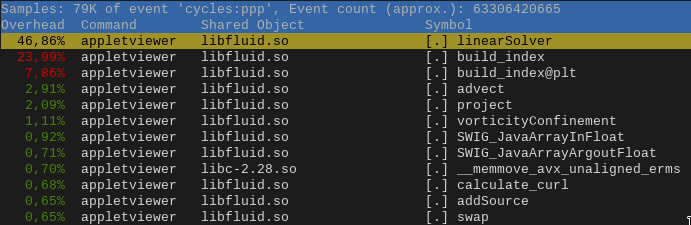
\includegraphics[scale=0.62]{figures/optims/gcc-O0/global.png}
    \caption{Profilage global avec \ac{GCC} en \enquote{-O0}}
    \label{fig.optim.global}
\end{figure}

Comme nous pouvions l’imaginer, la Figure~\ref{fig.optim.global} nous confirme
que les fonctions les plus chaudes sont \enquote{linearSolver()} et
\enquote{build\_index()}, la première de par sa nature de calcul intensif, la
deuxième du fait qu’elle soit appelée énormément de fois. On remarque que toutes
les autres fonctions sont d’une importance mineure dans le temps d’exécution du
programme : inférieure à $3\%$ pour la plus chaude. À elle seule, la fonction
\enquote{linearSolver()} prend presque $50\%$ du temps d’exécution du
programme : c’est la plus importante.

\begin{figure}
    \centering
    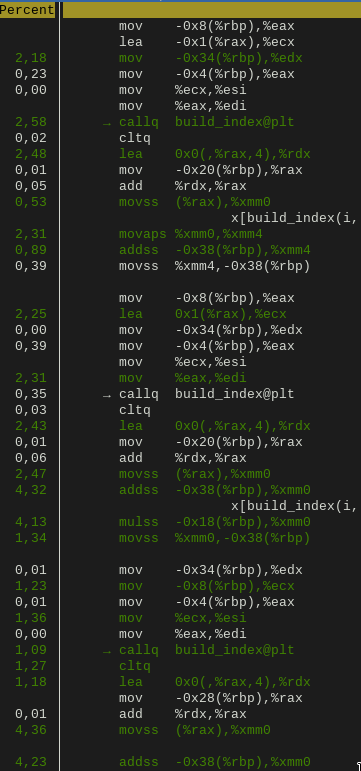
\includegraphics[scale=0.6]{figures/optims/gcc-O0/linearSolver-others.png}
    \\ \phantom{ } \\
    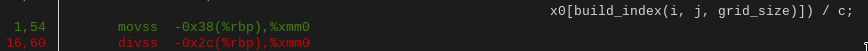
\includegraphics[scale=0.5]{figures/optims/gcc-O0/linearSolver-div.png}
    \caption{Profilage de \enquote{linearSolver()} avec \ac{GCC} en \enquote{-O0}}
    \label{fig.optim.linearSolver}
\end{figure}

La Figure~\ref{fig.optim.linearSolver} nous permet d'analyser quelles
instructions de la fonction \enquote{linearSolver()} ont un impact important sur
le temps d’exécution. La première image nous montre un lot successif
d’instructions prenant chacune 1 à 4\% du temps d’exécution : des \textit{add},
\textit{mul}, \textit{mov}, \textit{lea}. La deuxième image met en évidence une
instruction \textit{div} qui prends à elle seule $16\%$ du temps de la fonction.
On identifie donc parfaitement les deux sources de ralentissement de la
fonction : la première étant un trop grand nombre d’instructions pour effectuer
les calculs et la seconde étant la division.

\begin{figure}
    \centering
    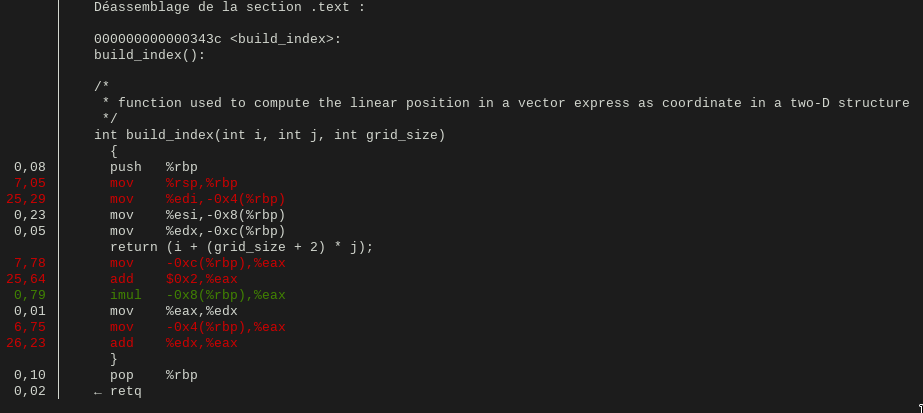
\includegraphics[scale=0.40]{figures/optims/gcc-O0/build_index.png}
    \\ \phantom{ } \\
    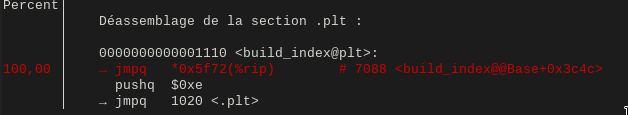
\includegraphics[scale=0.55]{figures/optims/gcc-O0/build_index@plt.png}
    \caption{Profilage de \enquote{build\_index()} et \enquote{build\_index()@plt} avec \ac{GCC} en \enquote{-O0}}
    \label{fig.optim.build_index}
\end{figure}

Le temps passé dans la fonction \enquote{build\_index()} est divisé
équitablement en \textit{mov}/\textit{add} d'après la
Figure~\ref{fig.optim.build_index}, permettant de faire les deux additions et la
multiplication que doit faire la fonction. On remarque tout de même que $32\%$
du temps de la fonction est passé dans la mise en place de la stack frame de la
fonction (2 premières instructions \textit{mov}). Enfin, on remarquera que $7\%$
du temps de la simulation est passée dans la fonction \enquote{build\_index@plt}.
Pour comprendre d’où vient cette fonction, il faut revenir sur les bases du
fonctionnement du chargement dynamique de code. Afin d’avoir des bibliothèques
partagées qui puissent être chargées qu’une seule fois en mémoire mais à des
emplacements indépendants pour deux processus différents, on utilise un
mécanisme de code à position indépendante (\ac{PIC}). Ce système fait recours à
une \ac{GOT} contenant les adresses des variables et fonctions dont
l’emplacement n’est pas connu au moment de la compilation. Cette \ac{GOT} est
consultée par les fonctions contenues dans la \ac{PLT}, une table contenant des
fonctions \textit{stubs} (wrapper) qui sont appelées à la place de la vraie
fonction. Cette fonction stub (@plt) permet d’aller consulter la \ac{GOT}, de
remplir la \ac{GOT} lors du premier appel (\textit{lazy loader}), enfin
d’exécuter la vraie fonction. Toutes les prochaines fois ou la fonction stub
sera appelée, alors on va directement charger l’adresse contenu dans la
\textit{GOT} pour appeler la fonction désirée.

\subsection{Mise en place de la compilation}
\label{sub.optim.compil}

Premièrement, nous avons testé les flags suivants activant des options de lot
d’optimisation : \enquote{-O1}, \enquote{-O2}, \enquote{-O3} (agressivité au
détriment de la taille du code généré), \enquote{-Os} (optimisation de la taille
du code). L’utilisation d’un de ces flags nous apporte une légère amélioration
de fluidité visuelle, cependant il se trouve que nous n’avons pas observé de
différence majeure entre ces 4 différentes flags, que ce soit en termes de code
généré ou de performances et répartition du temps entre les fonctions.
Ci-dessous les images des résultats avec \ac{GCC} et \enquote{-O2}.

\begin{figure}
    \centering
    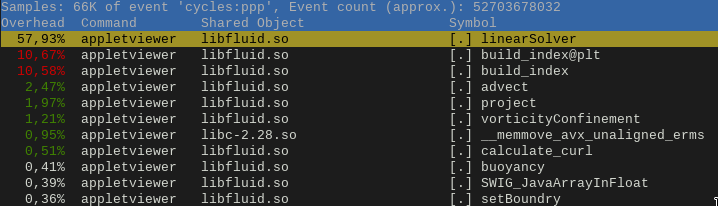
\includegraphics[scale=0.58]{figures/optims/gcc-O2/global.png}
    \caption{Profilage global avec \ac{GCC} en \enquote{-O2}}
    \label{fig.optim.compil.gcc.global}
\end{figure}

Au premier abord de la Figure~\ref{fig.optim.compil.gcc.global}, nous pourrions
être étonnés que la fonction \enquote{linearSolver()} soit passée de $46\%$ à
$57\%$, comme si l’optimisation par le compilateur l’avait rendu plus lente. En
fait il n’en est rien : on passe en effet plus de temps dans la fonction
\enquote{linearSolver()} car on passe moins de temps dans les autres fonctions,
ces dernières étant elles aussi optimisées. En effet, on voit que le temps passé
dans la fonction \enquote{build\_index()} est passé de $24\%$ à $10\%$. Enfin,
il en va de même pour le temps qui a augmenté de $3\%$ pour
\enquote{build\_index@plt} : puisque \enquote{build\_index()} est plus courte,
alors on passe autant de temps à appeler la fonction qu’à effectuer les calculs.

\begin{figure}
    \centering
    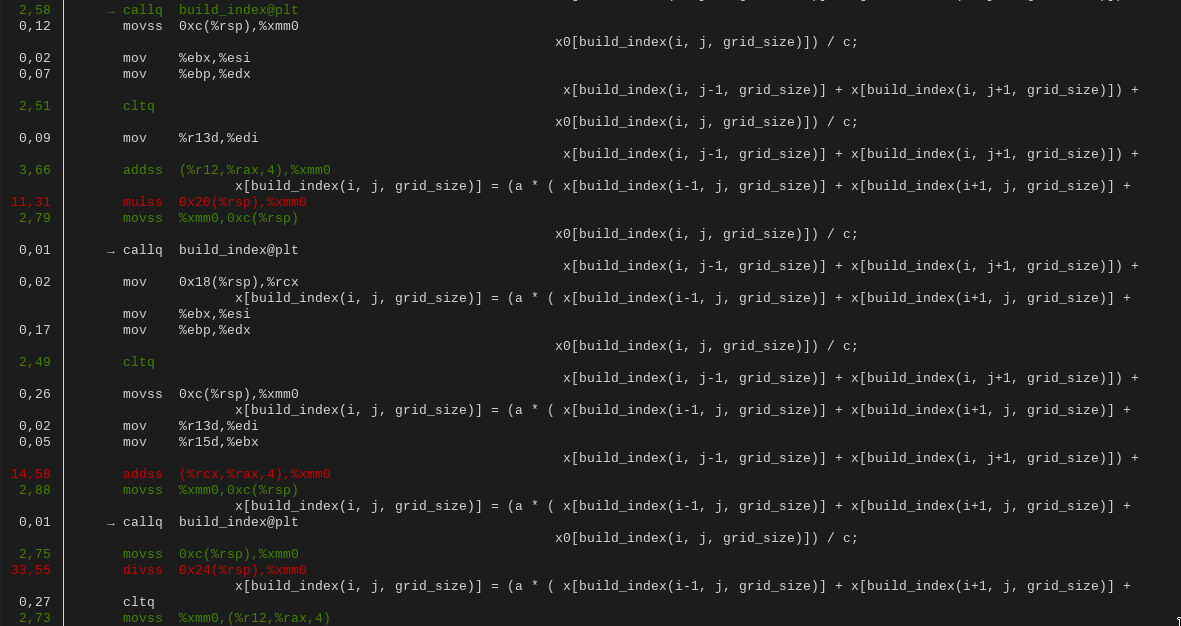
\includegraphics[scale=0.35]{figures/optims/gcc-O2/linearSolver.png}
    \caption{Profilage de \enquote{linearSolver()} avec \ac{GCC} en \enquote{-O2}}
    \label{fig.optim.compil.gcc.linearSolver}
\end{figure}

Concernant la fonction \enquote{linearSolver()} de la
Figure~\ref{fig.optim.compil.gcc.linearSolver}, on voit que le nombre
d’instructions à nettement été réduit. On est passé de beaucoup d’instruction
prenant chacune 1 à $4\%$ à quelques petites instructions et 3 instructions
principales de 10 à 33\%. Ce nouveau schéma permettra sans doute de mieux cibler
les instructions qui vont avoir besoin d’être optimisé.

\begin{figure}
    \centering
    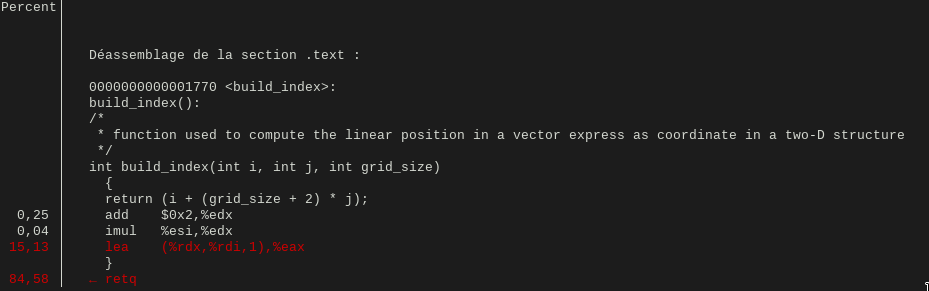
\includegraphics[scale=0.4]{figures/optims/gcc-O2/build_index.png}
    \caption{Profilage de \enquote{build\_index()} avec \ac{GCC} en \enquote{-O2}}
    \label{fig.optim.compil.gcc.build_index}
\end{figure}

Comme nous pouvons le constater sur la
Figure~\ref{fig.optim.compil.gcc.build_index}, le code a été considérablement
réduit et optimisé par le compilateur pour la fonction \enquote{build\_index()}.
En effet, une grande partie des instructions ont été supprimés car on utilise un
passage de valeur par registres (plus rapide) et non plus par la pile. De plus,
on utilise l’instruction \textit{lea} spécialisé dans le calcul d’adresse.
Finalement, il nous reste \textit{lea} qui prend 15\% de la fonction et le
retour de la fonction qui prend 85\% du temps.

Nous avons aussi testé les performances du programme avec
\enquote{Clang/\ac{LLVM}}, et les flags d’optimisation les plus agressifs
(\enquote{-03}). Ci-dessous les images des résultats avec Clang et \enquote{-O3}.

\begin{figure}
    \centering
    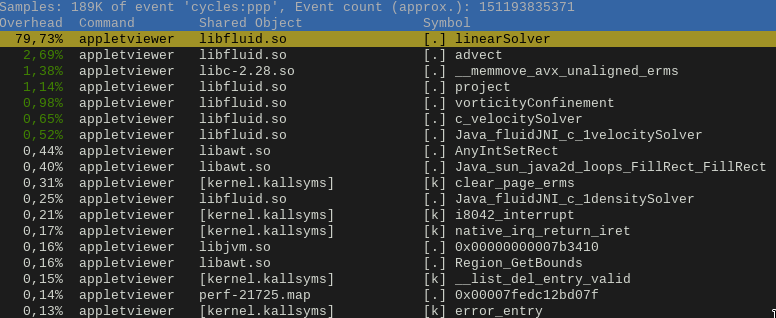
\includegraphics[scale=0.58]{figures/optims/clang-O3/global.png}
    \caption{Profilage global avec Clang en \enquote{-O3}}
    \label{fig.optim.compil.clang.global}
\end{figure}

Illustré par la Figure~\ref{fig.optim.compil.clang.global}, avec Clang et
les options de compilation les plus agressives, on voit que le temps passés dans
la fonction \enquote{linearSolver()} est passé de 57\% avec \ac{GCC} à 80\%.
Encore une fois, cela veux dire que les autres fonctions ont été encore plus
radicalement minimisées. On notera aussi les fonctions \enquote{build\_index()}
et \enquote{build\_index@plt} ont complètement été supprimés.

\begin{figure}
    \centering
    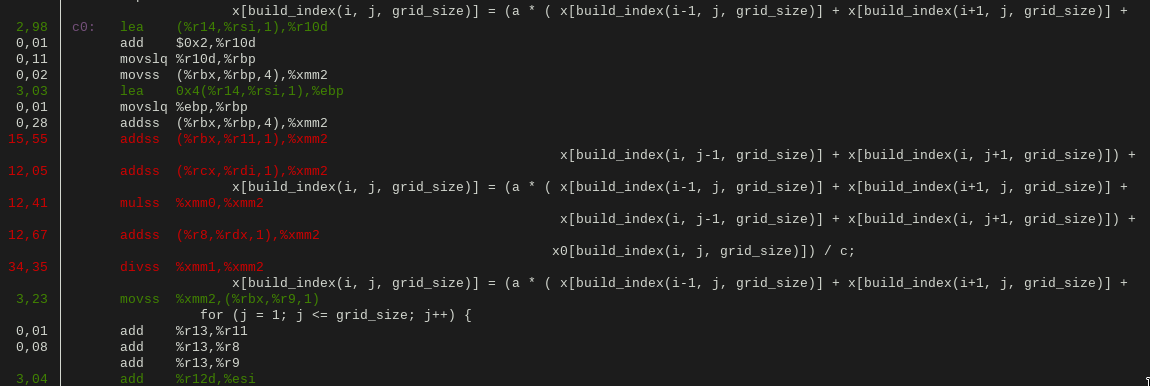
\includegraphics[scale=0.35]{figures/optims/clang-O3/linearSolver.png}
    \caption{Profilage de \enquote{linearSolver()} avec Clang en \enquote{-O3}}
    \label{fig.optim.compil.clang.linearSolver}
\end{figure}

Par la Figure~\ref{fig.optim.compil.clang.linearSolver}, nous observons que le
code de \enquote{linearSolver()} a été extrêmement réduit en 5 instructions
principales, introduites par \ac{SSE}. C’est vers ce genre de code que devrait
converger nos optimisations manuelles.

Nous observons donc un net gain à utiliser Clang par rapport à \ac{GCC}, qu'il
soit visuel ou factuel. Cependant, pour nous permettre d’appliquer des
optimisations vu en cours à la main, nous allons opter pour la version que
produit \ac{GCC} comme base de travail.

Enfin, nous noterons que nous avons aussi essayé d’utiliser l’option
d’optimisation \enquote{-Ofast} avec \ac{GCC}. Ce fut un succès visuel puisque
l’accélération était nettement présente, cependant nous avons préféré ne pas
laisser cette option activée : ce flag permet d’activer des optimisations
mathématiques, notamment sur les flottants, en autorisant des arrondis et le
non-respect de certains standards de l'\ac{IEEE}. N’ayant aucun moyen de vérifier par
nous même si les calculs sont encore de la précision voulue avec ce flag, nous
préférons ne pas tenter une opération qui pourrait remettre en cause la validité
de la simulation.

\subsection{Inlining}
\label{sub.optim.inlin}

Comme vu dans la section précédente, la fonction \enquote{build\_index()} était
très consommatrice en cycle (malgré l’optimisation du passage de paramètres par
les registres plutôt que par la pile) à cause de 2 phénomènes :
\begin{enumerate}
    \item L’appel de la fonction, qui passe par deux indirections du fait de la
        \ac{PLT}, nous fait exécuter des instructions supplémentaires.
    \item Les branchements dans le code ne favorise pas le principe de localité
        des caches.
\end{enumerate}

Une optimisation bien connue consiste donc à \textit{inliner} une fonction :
cela revient à remplacer automatiquement lors de la compilation, dans le code
généré du binaire, tous les appels à ladite fonction par le corps de la
fonction. Cela à pour avantage de réduire considérablement le temps
d’utilisation d’une fonction (plus de branchement ni de passage de paramètre).
Cependant, cela peux grossir de manière drastique la taille du code si la
fonction inliner est une longue fonction : ce qui n’est pas le cas ici, de toute
évidence.

Pour procéder à l’inlining, cela est très simple puisqu’il suffit de l’indiquer
au compilateur avec le mot clé approprié. On passe donc du code
suivant (Listing~\ref{lst.optim.inlin}) à la ligne 1 à celui de la ligne 2.

\begin{listing}[h]
    \begin{minted}[linenos,numbersep=5pt,frame=lines,framesep=2mm]{C}
int build_index(int i, int j, int grid_size)
inline int build_index(int i, int j, int grid_size)
    \end{minted}
    \caption{Fonction \enquote{build\_index()} avant et après inlining}
    \label{lst.optim.inlin}
\end{listing}

\begin{figure}
    \centering
    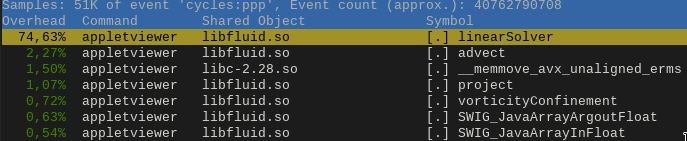
\includegraphics[scale=0.55]{figures/optims/inlining/global.png}
    \caption{Profilage global après inlining de la fonction \enquote{build\_index()}}
    \label{fig.optim.inlin.global}
\end{figure}

En termes de gain, la fluidité visuelle est grandement améliorée et tout de
suite remarquable grâce à l’inlining. Par le profilage globale
(Figure~\ref{fig.optim.inlin.global}), on peut observer que les fonctions
\enquote{build\_index()} et \enquote{build\_index@plt} ont été complètement
supprimées et que l’on est passé d’un temps de $56\%$ dans la fonction
\enquote{linearSolver()} à maintenant $74\%$, ce qui est bon signe : il faut
maintenant se concentrer sur l’optimisation de cette fonction.

\begin{figure}
    \centering
    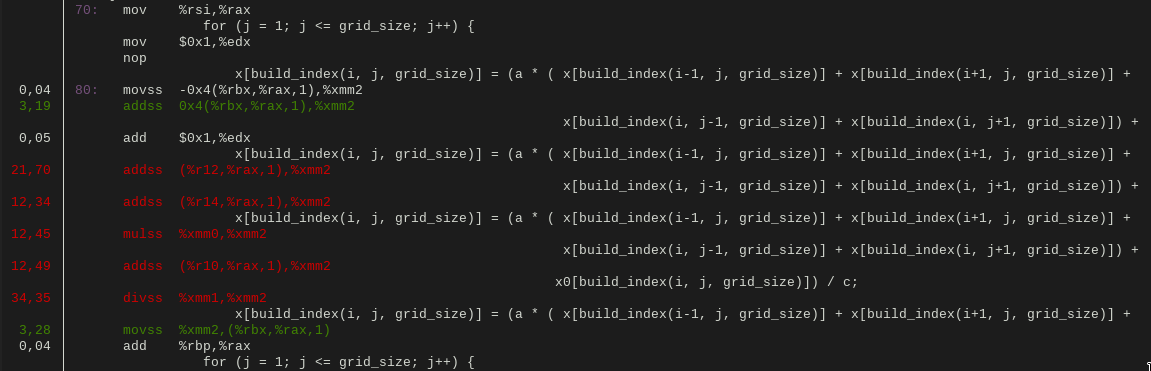
\includegraphics[scale=0.37]{figures/optims/inlining/linearSolver.png}
    \caption{Profilage de \enquote{linearSolver()} après inlining de la fonction \enquote{build\_index()}}
    \label{fig.optim.inlin.linearSolver}
\end{figure}

Concernant le code de la fonction \enquote{linearSolver()}, on observe dans la
Figure~\ref{fig.optim.inlin.linearSolver} qu’il a été considérablement réduit et
compacté, il ressemble maintenant fortement au code créer par Clang, décrit
dans la section précédente.

\subsection{Mots-clés appropriés}
\label{sub.optim.keywords}

Les mots-clés peuvent souvent faire une différence capitale dans le processus
d’optimisation du compilateur. En effet, de nombreuses optimisations ne peuvent
être effectuées que sous réserve de certaines conditions, par exemple : qu’une
variable ne soient pas modifié par un autre thread ou encore qu’une variable
soit constante. Nous disposons, en C, des mots-clés (entre autres)
\enquote{static} et \enquote{const} qui sont très utiles pour indiquer ce genre
de cas et bien d’autres encore. Après avoir appliqué le mot-clé \enquote{static}
à toutes les fonctions (hormis les 2 points d’entrée de la bibliothèque) afin
d’indiquer qu’elles sont locales au module compilé (améliorant par exemple
l’\textit{inlining} automatique) et le mot-clé \enquote{const} aux variables
constantes de la fonction \enquote{linearSolver()}, nous obtenons le résultat de
la Figure~\ref{fig.optim.keywords.global} au profilage.

\begin{figure}
    \centering
    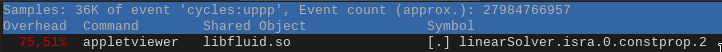
\includegraphics[scale=0.55]{figures/optims/keywords/global.png}
    \caption{Profilage global après ajouts des mots-clés appropriés}
    \label{fig.optim.keywords.global}
\end{figure}

Le suffix \enquote{.isra.constprop} signifie que \ac{GCC} à automatiquement
effectué une propagation de constante et/ou a retiré des paramètres inutiles. À
partir de cette information, nous nous sommes rapidement rendu compte qu’il y
avait des variables inutiles passées à \enquote{linearSolver()} : \enquote{$dt$}
n’était jamais utilisé, et \enquote{$b$} était toujours égal à 0. Nous avons
donc nous-mêmes supprimé ces variables dans la fonction.

Il n’y à pas de gain de performance visible ou mesurable, cependant cela
éclairci le code source et facilitera peut-être l’analyse du compilateur pour de
prochaines optimisations. 

\subsection{Modification des calculs}
\label{sub.optim.cacl}

Comme nous pouvions le voir dans les sections précédentes, ils nous faillait
maintenant nous concentrer sur le cœur de calcul de \enquote{linearSolver()}.
L’instruction la plus problématique était la division, suivi de la
multiplication puis des additions. Analysons la situation : pour cela, nous
avons déterminé les différentes valeurs que pouvait prendre les variables de la
fonction, puis nous avons affiché en temps réel les valeurs des variables avec
un compteur permettant de savoir combien de fois quelle variable à pris quelle
valeur.

\subsubsection{Multiplcation}
\label{sub.optim.calc.mul}

Nous avons d’abord analysé la variable \enquote{$a$}, celle qui se retrouve dans
la multiplication. Il se trouve que cette variable ne prend que les valeurs 1 ou
0 : il s’agit en réalité d’un booléen, bien que le type soit un float. Cette
variable multiplie une suite de 3 additions : si \enquote{$a$} est à 1, alors on
garde les 3 additions ; si la variable est à 0, alors il ne faut pas faire les
additions. De toute évidence, cette variable n’est là que pour contrôler le fait
de garder ou non les additions et n’est pas là pour effectuer une mise à
l’échelle par un facteur précis. Dès lors, si la variable est à 0, notre
programme va faire les 3 additions pour ensuite les multiplier avec 0 : c’est
une grosse perte de temps. On conseille souvent d’éviter les branchements dans
une boucle, mais il se trouve qu’ici, avoir un branchement (quelques cycles, 2 à
4) permettrait d’éviter :
\begin{enumerate}
    \item Pire des cas : 1 multiplication (quelques cycles, 2 à 4).
    \item Meilleur des cas : 1 multiplication et 3 additions (plus d’une
        dizaine de cycles, 10 à 15).
\end{enumerate}
Les cycles ont étés pris pour un processeur \textit{Sandy Bridge} sur les
documents d’\textbf{Agner Fog}. Un branchement permet donc clairement d’être
gagnant s’il est assez prédictible.

\begin{listing}
    \begin{minted}[linenos,numbersep=5pt,frame=lines,framesep=2mm]{C}
const int inv_a = !(int)a;
[...]
((inv_a ? 0 :
  ((x[build_index(i-1, j, grid_size)] + x[build_index(i+1, j, grid_size)]) +
   (x[build_index(i, j-1, grid_size)] + x[build_index(i, j+1, grid_size)]))
 ) + x0[build_index(i, j, grid_size)]
) / c;
    \end{minted}
    \caption{Résultat de la modification de la multiplication}
    \label{lst.optim.calc.mul}
\end{listing}

Nous avons donc procéder de la manière suivante, visible sur le
Listing~\ref{lst.optim.calc.mul} : nous faisons un \textit{NOT} de la variable
dans une autre variable, déclaré constante. Nous prenons garde à stocker le
résultat dans un \textit{int} et à faire un \textit{cast} au préalable : de
cette manière, \ac{GCC} va générer une instruction \textit{test} plutôt qu’une
instruction \textit{ucomiss} (plus coûteuse) pour effectuer la comparaison. Nous
stockons le \textit{NOT} dès le début de la fonction pour ne pas avoir à le
calculer à chaque itération de la boucle, et nous voulons le \textit{NOT} afin
de faire arriver le cas où \enquote{$a$} est à 0 en premier. En effet, nous
avons testé un grand nombre de scénarios pour trouver dans quelle configuration
le code généré et la prédiction de branchement fonctionnait au mieux :
\begin{enumerate} \item Tentative de faire intervenir le cas le plus fréquent en
            premier, puis en second. \item Utilisation de \textit{if-else} ou
            d’opérateur ternaire. \item Séparation du résultat dans une variable
            temporaire, ou calcul inliner. \item Utilisation d’un
                \textit{builtin} afin d’indiquer à \ac{GCC} la branche la plus
prise, ou de laisser totalement la main au processeur. \end{enumerate} Il se
trouve que finalement, la combinaison qui fonctionnait de manière la plus
optimale possible se trouve être : \begin{enumerate} \item Le cas le plus
        fréquent en premier. \item Utilisation d’un opérateur ternaire. \item
        Calcul \textit{inliner}. \item Ne pas indiquer à \ac{GCC} la branche la
            plus souvent prise (le \acs{CPU} se débrouille très bien tout seul
!). \end{enumerate}

À noter que pour les 3 additions, nous les avons regroupés depuis la forme $(a +
b + c + d)$ vers la forme $((a + b) + (c + d))$. Cela permet d’expliciter la
non-dépendance des opérations dans cette chaîne, et ainsi de laisser le
\acs{CPU} commencer le calcul de $(c + d)$ avant la fin de $(a + b)$.

\subsubsection{Division}
\label{sub.optim.calc.div}

La deuxième optimisation majeure est la suppression de la division. Comme vu sur
la Figure~\ref{fig.optim.inlin.linearSolver}, la division prenait un peu plus de
$30\%$ du temps d’exécution de notre fonction, ce qui est énorme. Nous avons
donc analyser la variable \enquote{$c$} : il se trouve que cette variable prends
la valeur 1 avec une probabilité de $\frac{2}{3}$ et la valeur 4 avec une
probabilité de $\frac{1}{3}$. Diviser par 1 revient à ne pas diviser, et diviser
par 4 reviens à multiplier par $0,25$. Nous calculons donc l’inverse de la
variable au début de la fonction, et nous multiplions le tout par cette variable
plutôt que d’effectuer une division coûteuse à chaque itération : soit on
multiplie par 1, soit on multiplie par $0.25$. Ici, l’utilisation d’un
branchement pour ne pas multiplier lorsque \enquote{$c$} est égal à 1 était tout
aussi coûteux que de multiplier par 1, donc inutile.

\begin{listing}
    \begin{minted}[linenos,numbersep=5pt,frame=lines,framesep=2mm]{C}
const float inv_c = 1. / c;
[...]
((inv_a ? 0 :
  ((x[build_index(i-1, j, grid_size)] + x[build_index(i+1, j, grid_size)]) +
   (x[build_index(i, j-1, grid_size)] + x[build_index(i, j+1, grid_size)]))
 ) + x0[build_index(i, j, grid_size)]
) * inv_c;
    \end{minted}
    \caption{Résultat de la suppression de la division}
    \label{lst.optim.calc.div}
\end{listing}

\subsubsection{Invariants}
\label{sub.optim.calc.inv}

\begin{listing}
    \begin{minted}[linenos,numbersep=5pt,frame=lines,framesep=2mm]{C}
const float tmp1 = -0.5f * (1. / grid_size);
const float tmp2 = 0.5f * grid_size;
[...]
for (j = 1; j <= grid_size; j++) {
    div[build_index(i, j, grid_size)] = tmp1 * (x[build_index(i+1, j,
        grid_size)] - [...]);
}
[...]
for (j = 1; j <= grid_size; j++) {
    x[build_index(i, j, grid_size)] -= tmp2 * [...];
    y[build_index(i, j, grid_size)] -= tmp2 * [...];
}
    \end{minted}
    \caption{Calcul préalable d'invariants de boucle}
    \label{lst.optim.calc.inv}
\end{listing}

Nous avons procédés à quelques légères optimisations dans la fonction
\enquote{project()} : en effet, des invariants de boucle étaient présents et
pouvaient être pré-calculé. Un invariant de boucle est, ici, un groupe de calcul
calculé à chaque itération inutilement alors qu’il pourrait être calculé avant
ladite boucle. Vous pouvez observer l’optimisation sur le
Listing~\ref{lst.optim.calc.inv}.

\subsubsection{Résultat}
\label{sec.optim.calc.res}

\begin{figure}
    \centering
    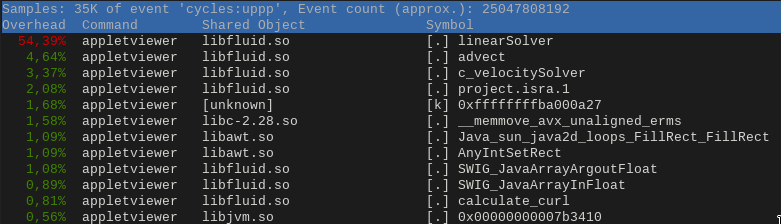
\includegraphics[scale=0.55]{figures/optims/computing/global.png}
    \caption{Profilage global après modifications des calculs}
    \label{fig.optim.calc.global}
\end{figure}

\begin{figure}
    \centering
    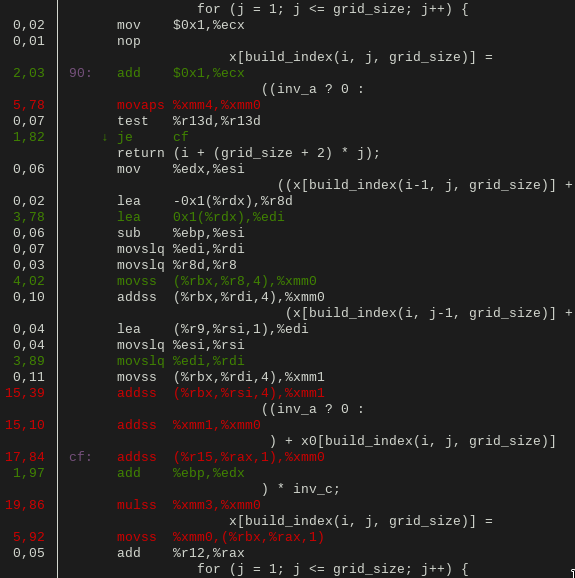
\includegraphics[scale=0.55]{figures/optims/computing/linearSolver.png}
    \caption{Profilage de \enquote{linearSolver()} après modifications des calculs}
    \label{fig.optim.calc.linearSolver}
\end{figure}

Tout d’abord, d’expérience utilisateur, ces optimisations sont un franc succès.
Le mode de résolution \enquote{255x255} peut enfin être utilisé sur
notre machine de test de manière tout à fait confortable, avec environ 60 images
par secondes (ressentit).

Sur la Figure~\ref{fig.optim.calc.global}, on observe un net changement de
répartition de temps de calcul : \enquote{linearSolver()}, qui prenant
auparavant $75\%$ du programme, n’en prends maintenant que $54\%$ ! On obtient
donc un gain d’environ $20\%$, ce qui est non-négligeable.

Sur la Figure~\ref{fig.optim.calc.linearSolver}, on peut observer nos
changements effectués : un \textit{mul} a disparu, le \textit{div} a été
remplacé par un \textit{mul}, un \textit{test} et un \textit{je} sont apparu...
De nouvelles instructions qui ont la même fonction que les anciennes, mais qui
consomment moins de temps.

\subsection{Mémoire cache}
\label{sub.optim.cache}

\begin{figure}
    \centering
    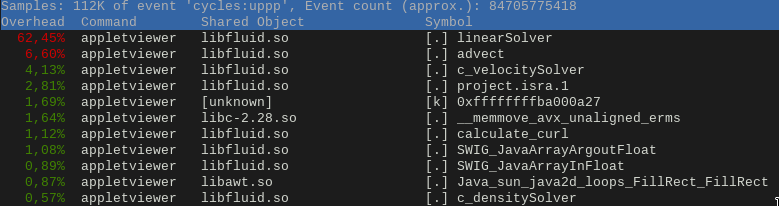
\includegraphics[scale=0.50]{figures/optims/cache/global-before.png}
    \caption{Profilage global avant opitmisation du cache}
    \label{fig.optim.cache.before}
\end{figure}

\begin{figure}
    \centering
    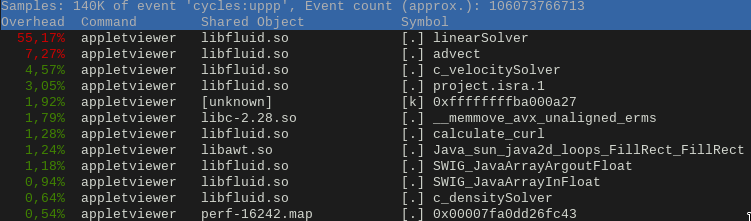
\includegraphics[scale=0.55]{figures/optims/cache/global-after.png}
    \caption{Profilage global après opitmisation du cache}
    \label{fig.optim.cache.after}
\end{figure}

Maintenant que la simulation fonctionne de manière très satisfaisante avec une
résolution de \enquote{225x225}, nous passons nos mesures sur la résolution
\enquote{450x450}, qui n’est toujours pas fluide. Nous pouvons observer le
résultat de la mesure avant la prochaine optimisation sur la
Figure~\ref{fig.optim.cache.before} : notre fonction \enquote{linearSolver()}
prends $62\%$ de notre temps d’exécution.

Dans cette partie, nous avons essayé d’optimiser l’utilisation de la mémoire
cache en améliorant la localité des accès à la mémoire. Pour cela, deux
techniques ont été mises en œuvres :
\begin{enumerate}
    \item Inversion des deux boucles.
    \item Cache Blocking.
\end{enumerate}

Pour la première technique, il s’agit d’inverser l’ordre des boucles intérieur
et extérieur $(i \text{ et } j)$ afin de parcourir les matrices par lignes et
non par colonnes. Plus la matrice sera grande (et ne rentrera plus entièrement
dans la mémoire cache), plus l’amélioration sera visible.

\begin{figure}
    \centering
    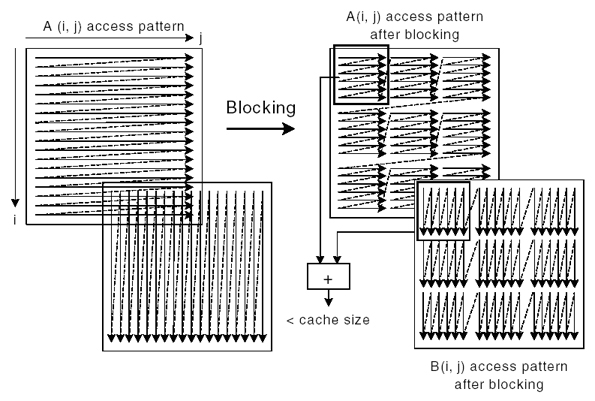
\includegraphics[scale=0.5]{figures/optims/cache/intel.jpg}
    \caption{Explication de l'effet du cache blocking (source : Intel.com)}
    \label{fig.optim.cache.intel}
\end{figure}

Pour la seconde technique, il s’agit de traiter la matrice par bloc carré plutôt
que la traiter complètement d’un seul coup. Le schéma de la
Figure~\ref{fig.optim.cache.intel} nous explique le principe très intuitivement.
Le but de cette manœuvre est de faire tenir le bloc traité dans la mémoire cache
et ainsi d’avoir un minimum de \textit{cache miss}. Si on traite la matrice
ligne par ligne mais qu’une ligne est plus grosse que la mémoire cache, alors à
chaque changement de ligne nous aurions des \textit{cache miss} inutiles. Une
chose important dans le cache blocking est la taille d’un bloc. Le déterminer de
manière peut-être une tâche assez ardue dû au décalage entre la théorie et la
pratique. Dans notre cas, nous l’avons déterminé de manière empirique en
effectuant plusieurs tests sur notre machine.

Ces deux techniques nous ont permis d’obtenir un léger gain en
\enquote{450x450}, illustré par la Figure~\ref{fig.optim.cache.after} : nous
pouvons voir que nous gagnons à peu $7\%$ de temps passé dans la fonction grâce
à l’optimisation de la mémoire. Si les matrices traités étaient beaucoup plus
grosses, alors le gain serai beaucoup plus visible. En revanche, si les matrices
deviennent très petite, alors cette optimisation nous fait perdre du temps dans
les contrôles de boucle.

Le résultat final de l’optimisation se résume par le code du Listing~\ref{lst.optim.cache}.
\begin{listing}[h]
    \begin{minted}[linenos,numbersep=5pt,frame=lines,framesep=2mm]{C}
#define BLOCK_SIZE 8
[...]
for (j = 1; j <= grid_size; j += BLOCK_SIZE) {
    for (i = 1; i <= grid_size; i += BLOCK_SIZE) {
        for (jj = j; jj <= j + BLOCK_SIZE && jj <= grid_size; jj++) {
            for (ii = i; ii <= i + BLOCK_SIZE && ii <= grid_size ; ii++) {
                x[build_index(ii, jj, grid_size)] = [...]
    \end{minted}
    \caption{Cache blocking et inversion des boucles}
    \label{lst.optim.cache}
\end{listing}

\subsection{Déroulage de boucle}
\label{sub.optim.unrol}

TODO

\subsection{Vectorisation}
\label{sub.optim.vec}

TODO

\subsection{Parallélisation}
\label{sub.optim.parall}

TODO

\section{Conclusion}
\label{sec.conc}

TODO

\newpage
\section*{Acronymes}
\label{sec.acro}

\begin{acronym}
    \acro{GCC}  {GNU Compiler Collection}
    \acro{LLVM} {Low Level Virtual Machine}
    \acro{PIC}  {Position-Independent Code}
    \acro{GOT}  {Global Offset Table}
    \acro{PLT}  {Procedure Linkage Table}
    \acro{AVX}  {Advanced Vector Extensions}
    \acro{SSE}  {Streaming SIMD Extensions}
    \acro{IEEE} {Institute of Electrical and Electronics Engineers}
    \acro{CPU}  {Central Processing Unit}
\end{acronym}

\end{document}
